\documentclass{beamer}
\usepackage{amsmath,amsbsy,amsopn,amstext,amsfonts,amssymb}
\usepackage{isomath}
\usepackage{ulem}
%\linespread{1.6}  % double spaces lines
\usepackage{graphicx}
\usepackage{subfigure}
\usepackage{color}
\usepackage{optidef}  % define optimization problems
\usepackage{multicol}  % multiple columns
\usepackage{listings} % for python code
\usepackage{mathrsfs}

\usepackage{polynom}
\newcommand{\adj}{\mathrm{adj}}
\newcommand{\constrainedmin}[3]{
		\begin{mini*}|s|
		{#2}{#1}{}{}
		\addConstraint{#3}
		\end{mini*}
}

\newcommand{\rwbcomment}[1]{{\color{blue}RWB:#1}}
\newcommand{\defeq}{\stackrel{\triangle}{=}}
\newcommand{\abs}[1]{\left|#1\right|}
\newcommand{\norm}[1]{\left\|#1\right\|}
\newcommand{\iprod}[1]{\left<#1\right>}
\newcommand{\ellbf}{\boldsymbol{\ell}}
\newcommand{\nubf}{\boldsymbol{\nu}}
\newcommand{\mubf}{\boldsymbol{\mu}}
\newcommand{\abf}{\mathbf{a}}
\newcommand{\bbf}{\mathbf{b}}
\newcommand{\cbf}{\mathbf{c}}
\newcommand{\dbf}{\mathbf{d}}
\newcommand{\ebf}{\mathbf{e}}
\newcommand{\fbf}{\mathbf{f}}
\newcommand{\gbf}{\mathbf{g}}
\newcommand{\hbf}{\mathbf{h}}
\newcommand{\ibf}{\mathbf{i}}
\newcommand{\jbf}{\mathbf{j}}
\newcommand{\kbf}{\mathbf{k}}
\newcommand{\lbf}{\mathbf{l}}
\newcommand{\mbf}{\mathbf{m}}
\newcommand{\nbf}{\mathbf{n}}
\newcommand{\obf}{\mathbf{o}}
\newcommand{\pbf}{\mathbf{p}}
\newcommand{\qbf}{\mathbf{q}}
\newcommand{\rbf}{\mathbf{r}}
\newcommand{\sbf}{\mathbf{s}}
\newcommand{\tbf}{\mathbf{t}}
\newcommand{\ubf}{\mathbf{u}}
\newcommand{\vbf}{\mathbf{v}}
\newcommand{\wbf}{\mathbf{w}}
\newcommand{\xbf}{\mathbf{x}}
\newcommand{\ybf}{\mathbf{y}}
\newcommand{\zbf}{\mathbf{z}}
\newcommand{\Jbf}{\mathbf{J}}
\newcommand{\Acal}{\mathcal{A}}
\newcommand{\Bcal}{\mathcal{B}}
\newcommand{\Lcal}{\mathcal{L}}
\newcommand{\Ncal}{\mathcal{N}}
\newcommand{\Rcal}{\mathcal{R}}
\definecolor{darkolivegreen}{rgb}{0.33, 0.42, 0.18}

\makeatletter
\newenvironment<>{proofstart}[1][\proofname]{%
    \par
    \def\insertproofname{#1\@addpunct{.}}%
    \usebeamertemplate{proof begin}#2}
  {\usebeamertemplate{proof end}}
\newenvironment<>{proofcont}{%
  \setbeamertemplate{proof begin}{\begin{block}{}}
    \par
    \usebeamertemplate{proof begin}}
  {\usebeamertemplate{proof end}}
\newenvironment<>{proofend}{%
    \par
    \pushQED{\qed}
    \setbeamertemplate{proof begin}{\begin{block}{}}
    \usebeamertemplate{proof begin}}
  {\popQED\usebeamertemplate{proof end}}
\makeatother

\title{ECEn 671: Mathematics of Signals and Systems}
\author{Randal W. Beard}
\institute{Brigham Young University}
\date{\today}

\begin{document}

%-------------------------------
\begin{frame}
	\titlepage
\end{frame}

%%%%%%%%%%%%%%%%%%%%%%%%%%%%%%%%%%%%%%%%%%%%%%%%%%%%%%%%%%%%%%%%%
\section{Matrix Condition Number}
\frame{\sectionpage}

%----------------------------------
\begin{frame}\frametitle{Matrix Condition Number}
	\begin{itemize}
	\item 	Suppose that $A \in \mathbb{C}^{n \times n}$ is full rank and $A^{-1}$ is to be computed numerically.  How reliable is the computation?
	\item $Ax = b$ can be written as 
		\[
			\begin{pmatrix}
   	 			a_{11} & \cdots & a_{1n}\\
    			\vdots & \ddots & \vdots\\
    			a_{n1} & \cdots & a_{nn}
    		\end{pmatrix}
    		\begin{pmatrix}
    			x_1 \\ \vdots \\ x_n
    		\end{pmatrix}
			=
			\begin{pmatrix}
				b_1 \\ \vdots \\ b_n	
			\end{pmatrix}
		\]
	\item Therefore, the solution $x$ is the intersection of $n-$ hyperplanes:
		\begin{align*}
		a_{11}x_1 + \ldots + a_{1n}x_n &= b_1\\
		\vdots\\
		a_{n1}x_1 + \ldots + a_{nn}x_n &= b_n
		\end{align*}
	\end{itemize}
\end{frame}

%----------------------------------
\begin{frame}\frametitle{Matrix Condition Number, cont.}
	\begin{itemize}
		\item The problem comes when these hyperplanes are almost parallel.
		\item In two dimensions we have two lines
			\begin{align*}
				a_{11}x_1 + a_{12}x_2 &= b_1\\
				a_{21}x_1 + a_{22}x_2 &= b_2
			\end{align*}
			which can be rewritten as
			\begin{align*}
  				x_2 &= -\frac{a_{11}}{a_{12}}x_1 + \frac{b_1}{a_{12}}\\
  				x_2 &= \underbrace{-\frac{a_{21}}{a_{22}}}_{\text{slope}}x_1 + \underbrace{\frac{b_2}{a_{22}}}_{\text{x-intercept}} 
			\end{align*}
	\end{itemize}
\end{frame}

%----------------------------------
\begin{frame}\frametitle{Matrix Condition Number, cont.}
	\begin{center}
		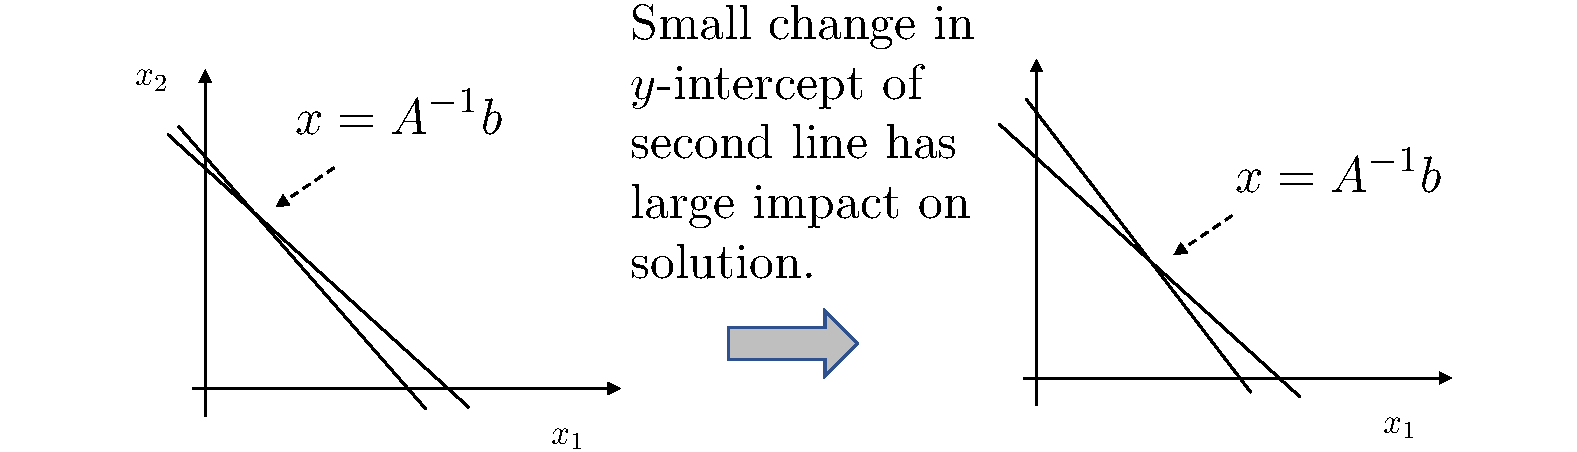
\includegraphics[width=\textwidth]{figures/chap4_condition_number}
	\end{center}
	If the two lines are almost parallel then small changes in the slope or $x_2$-intercept of either line will result in large changes in $x = A^{-1}b$.
\end{frame}

%----------------------------------
\begin{frame}\frametitle{Matrix Condition Number, cont.}
	\begin{itemize}
		\item Since computers must represent numbers to finite precision, representation errors could significantly change the numerical solution to the equation $Ax = b$.
		\item The condition number quantifies this effect.
	\end{itemize}
	
	\begin{definition}
		The condition number of a square matrix is defined to be
		\[ \mathcal{K}(A) = \norm{A }\norm{A^{-1} } \]
		where $\norm{\cdot }$ is an induced matrix norm usually taken to be the induced 2-norm.
	\end{definition}
\end{frame}

%----------------------------------
\begin{frame}\frametitle{Matrix Condition Number: Derivation}
	\begin{itemize}
		\item Given the two equations $Ax = b$ and $(A + \epsilon E)x = b$ where $\epsilon E$ is a ``small'' perturbation of $A$ (introduced by finite machine precision of $A$)
		\item Let $x_0 = A^{-1}b$ and
			\begin{align*}
				x_E &= (A + \epsilon E)^{-1}b\\
				&= [A(I + \epsilon A^{-1}E)]^{-1}b\\
				&= (I+\epsilon A^{-1}E)^{-1}A^{-1}b \\
				&= \underbrace{(I+\epsilon A^{-1}E)^{-1}}_{\text{perturbation}}x_0
			\end{align*}
	\end{itemize}
\end{frame}

%----------------------------------
\begin{frame}\frametitle{Matrix Condition Number: Derivation, cont.}
	Using the Neumann expansion gives
	$(I+\epsilon A^{-1}E)^{-1} = \displaystyle \sum_{i=0}^{\infty} (-\epsilon A^{-1} E)^i$.  Therefore
	\begin{align*}
		x_E &= (I+\epsilon A^{-1}E)^{-1}A^{-1}b \\ 
		&=(I - \epsilon A^{-1} E)A^{-1}b + O(\norm{\epsilon E }^2x_0)\\
		&= A^{-1}b - \epsilon A^{-1}EA^{-1}b + O(\norm{\epsilon E }^2x_0)\\
		&= x_0 - \epsilon A^{-1}Ex_0 + O(\norm{\epsilon E }^2x_0)
	\end{align*}
	Therefore
	\[\underbrace{\displaystyle\frac{\norm{x_E-x_0 }}{\norm{x_0 }}}_{\text{relative change in the solution}} \leq \underbrace{\epsilon\norm{A^{-1} }\norm{E }}_{\text{want to relate to relative change in $A$}}+O(\norm{\epsilon E }^2)  \]
\end{frame}

%----------------------------------
\begin{frame}\frametitle{Matrix Condition Number: Derivation, cont.}
	What is the relative change in $A$?
	\[\frac{  \norm{A - (A + \epsilon E) }}{  \norm{A }} = \frac{  \epsilon\norm{E }}{  \norm{A }} \defeq \rho\]
	Therefore
	\[
		\frac{ \norm{x_E - x_0 }}{\norm{x_0 }} \leq \rho \underbrace{\norm{A^{-1}}\norm{A } }_{\mathcal{K}(A)} + O(\norm{\epsilon E }^2) 
	\]
	
	The condition number $\mathcal{K}(A)$ relates (approximately) the relative change in $A$ to the relative change in the solution $x_0$.
\end{frame}

%----------------------------------
\begin{frame}\frametitle{Matrix Condition Number: Implication}
	\underline{Rule of Thumb:} \\
	If the solution is computed to $n$ digits then only
	\[ n - \log_{10} \mathcal{K}(A) \]
	can be considered to be accurate.
\end{frame}




\end{document}